\documentclass[tikz, border=6pt]{standalone}
\usepackage[T1]{fontenc}
\usepackage{lmodern}
\usepackage{amsmath,amssymb,bm}
\usepackage[scaled=0.95]{helvet}
\usetikzlibrary{arrows.meta}
\definecolor{Blue}{HTML}{3A76D8}
\definecolor{Green}{HTML}{3BA55C}
\definecolor{Orange}{HTML}{EE8133}
\definecolor{Purple}{HTML}{8459D1}
\definecolor{Ink}{HTML}{1F2937}
\begin{document}
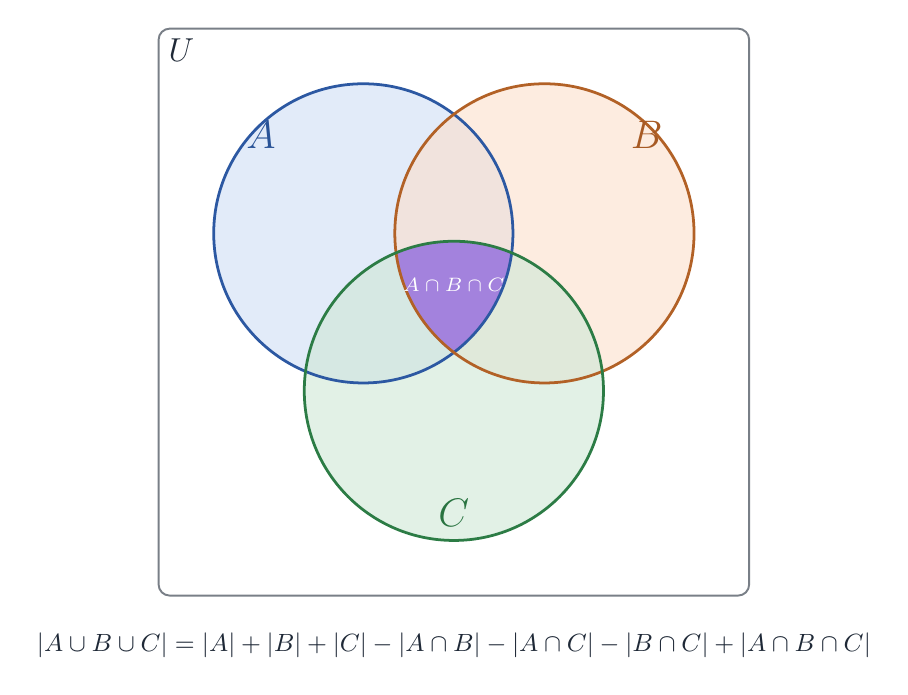
\begin{tikzpicture}[color=Ink, execute at begin picture={\sffamily}, line width=0.6pt, >={Stealth[length=5.5pt, width=4pt, inset=1.2pt]}, line join=round]
  \draw[draw=Ink!60, line width=0.7pt, rounded corners=4pt] (-2.6,-4) rectangle (4.9,3.2);
  \node[anchor=north west, font=\large] at (-2.6,3.2) {$U$};
  \draw[fill=Blue!25, draw=none, fill opacity=0.6] (0,0.6) circle[radius=1.9cm];
  \draw[fill=Orange!25, draw=none, fill opacity=0.6] (2.3,0.6) circle[radius=1.9cm];
  \draw[fill=Green!25, draw=none, fill opacity=0.6] (1.15,-1.4) circle[radius=1.9cm];
  \begin{scope}
    \clip (0,0.6) circle[radius=1.9cm];
    \clip (2.3,0.6) circle[radius=1.9cm];
    \draw[fill=Purple!75, draw=none] (1.15,-1.4) circle[radius=1.9cm];
  \end{scope}
  \draw[draw=Blue!75!black, line width=1pt] (0,0.6) circle[radius=1.9cm];
  \draw[draw=Orange!75!black, line width=1pt] (2.3,0.6) circle[radius=1.9cm];
  \draw[draw=Green!75!black, line width=1pt] (1.15,-1.4) circle[radius=1.9cm];
  \node[font=\Large, text=Blue!70!black] at (-1.3,1.85) {$A$};
  \node[font=\Large, text=Orange!70!black] at (3.6,1.85) {$B$};
  \node[font=\Large, text=Green!70!black] at (1.15,-2.95) {$C$};
  \node[font=\scriptsize, text=white] at (1.15,-0.05) {$A\cap B\cap C$};
  \node[anchor=north, font=\small] at (1.15,-4.35) {$|A\cup B\cup C| = |A|+|B|+|C|-|A\cap B|-|A\cap C|-|B\cap C|+|A\cap B\cap C|$};
\end{tikzpicture}
\end{document}
